% Created 2017-02-22 Wed 11:51
% Intended LaTeX compiler: pdflatex
\documentclass[presentation]{beamer}
\usepackage[utf8]{inputenc}
\usepackage[T1]{fontenc}
\usepackage{graphicx}
\usepackage{grffile}
\usepackage{longtable}
\usepackage{wrapfig}
\usepackage{rotating}
\usepackage[normalem]{ulem}
\usepackage{amsmath}
\usepackage{textcomp}
\usepackage{amssymb}
\usepackage{capt-of}
\usepackage{hyperref}
\usetheme{Madrid}
\author{Clarissa Littler}
\date{\today}
\title{If all math was computable\ldots{}}
\hypersetup{
 pdfauthor={Clarissa Littler},
 pdftitle={If all math was computable\ldots{}},
 pdfkeywords={},
 pdfsubject={},
 pdfcreator={Emacs 24.5.1 (Org mode 9.0.3)}, 
 pdflang={English}}
\begin{document}

\maketitle


\section{Talk}
\label{sec:org2e66927}

\begin{frame}[label={sec:orge0c899c}]{You wake up}
\end{frame}
\begin{frame}[label={sec:org6560e10}]{Programming class}
\begin{block}{}
\end{block}
\end{frame}
\begin{frame}[label={sec:orgbc548ad}]{Anti-virus}
\begin{block}{A virus is a self-replicating program}
\end{block}
\end{frame}

\begin{frame}[label={sec:org66acbfc}]{The new Hello World}
\begin{block}{Travelling Salesman}
\begin{center}
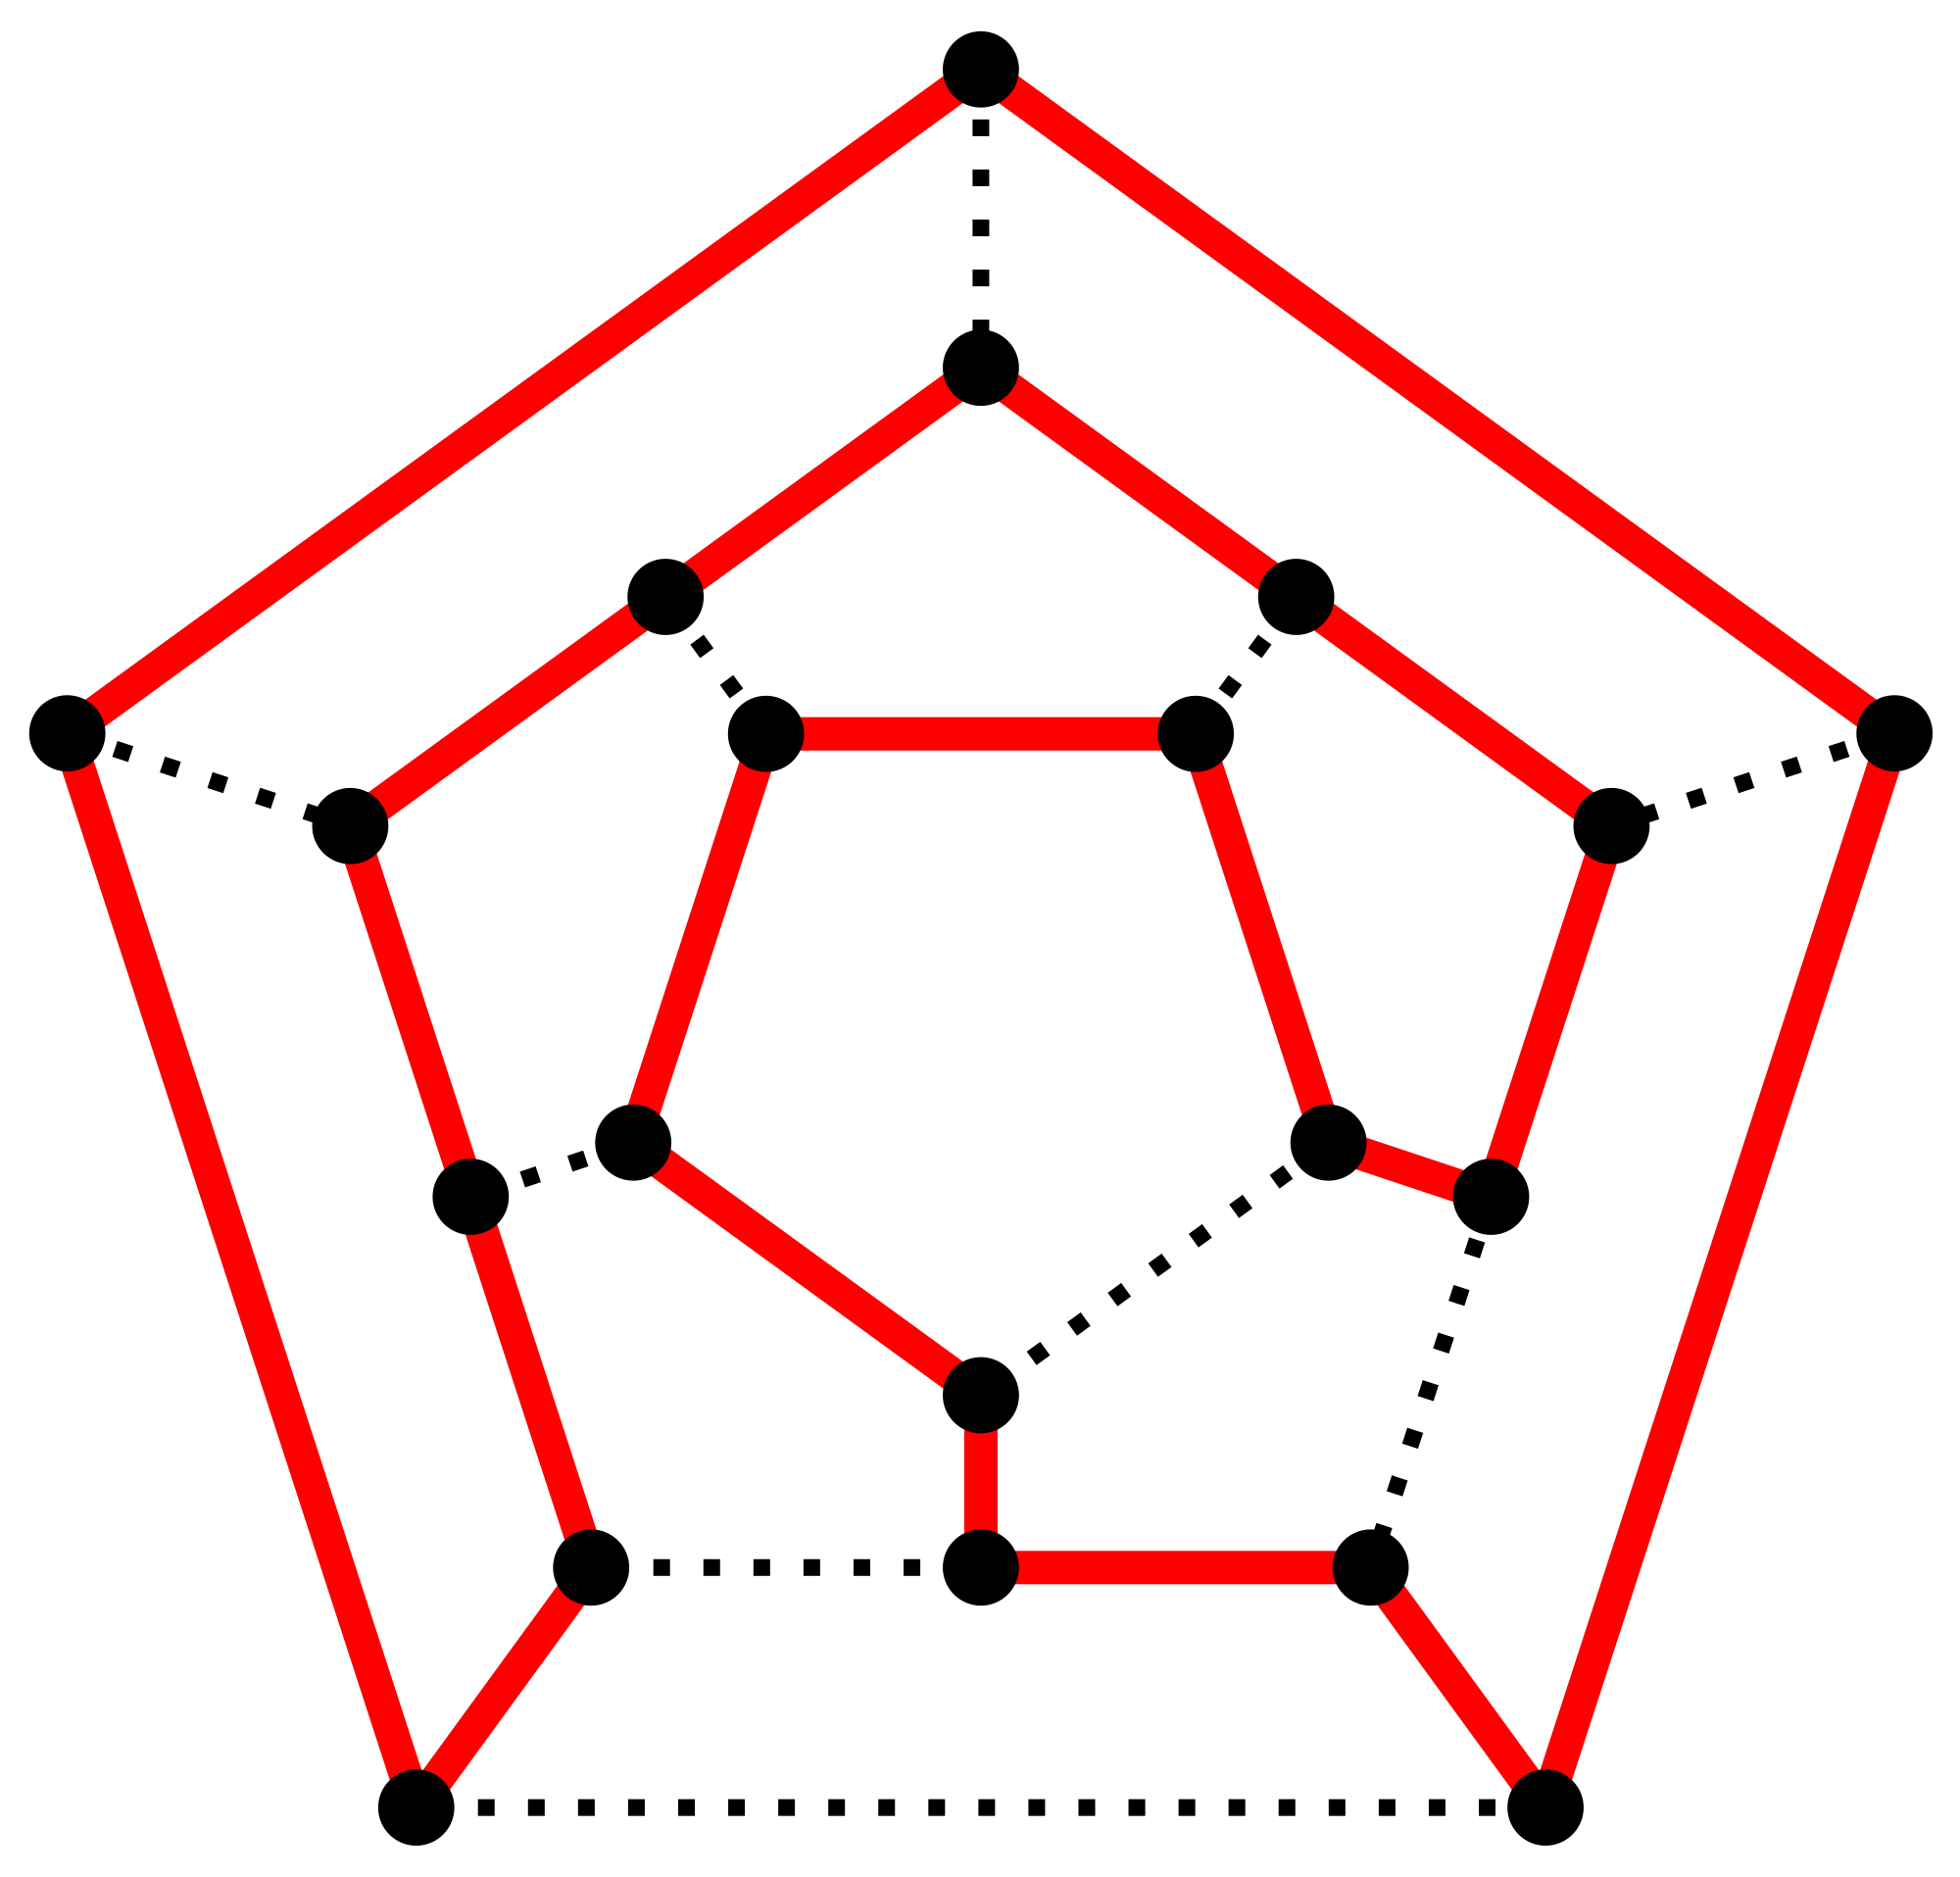
\includegraphics[width=.9\linewidth]{2000px-Hamiltonian_path.svg.png}
\end{center}
\end{block}
\end{frame}
\begin{frame}[label={sec:orge85e13e}]{Banking}
\begin{block}{Dedicated lines}
\begin{center}

\includegraphics[width=.9\linewidth]{Telegraph_Cable_Office.jpg}
\end{center}
\end{block}
\end{frame}
\begin{frame}[label={sec:org3aa09b8}]{Who uses passwords?}
\begin{block}{}
\end{block}
\end{frame}
\begin{frame}[label={sec:org7667ee8}]{Choice}
\end{frame}
\begin{frame}[label={sec:org7047978}]{Reverse engineering}
\end{frame}
\begin{frame}[label={sec:org275239c}]{Intellectual property}
\begin{center}
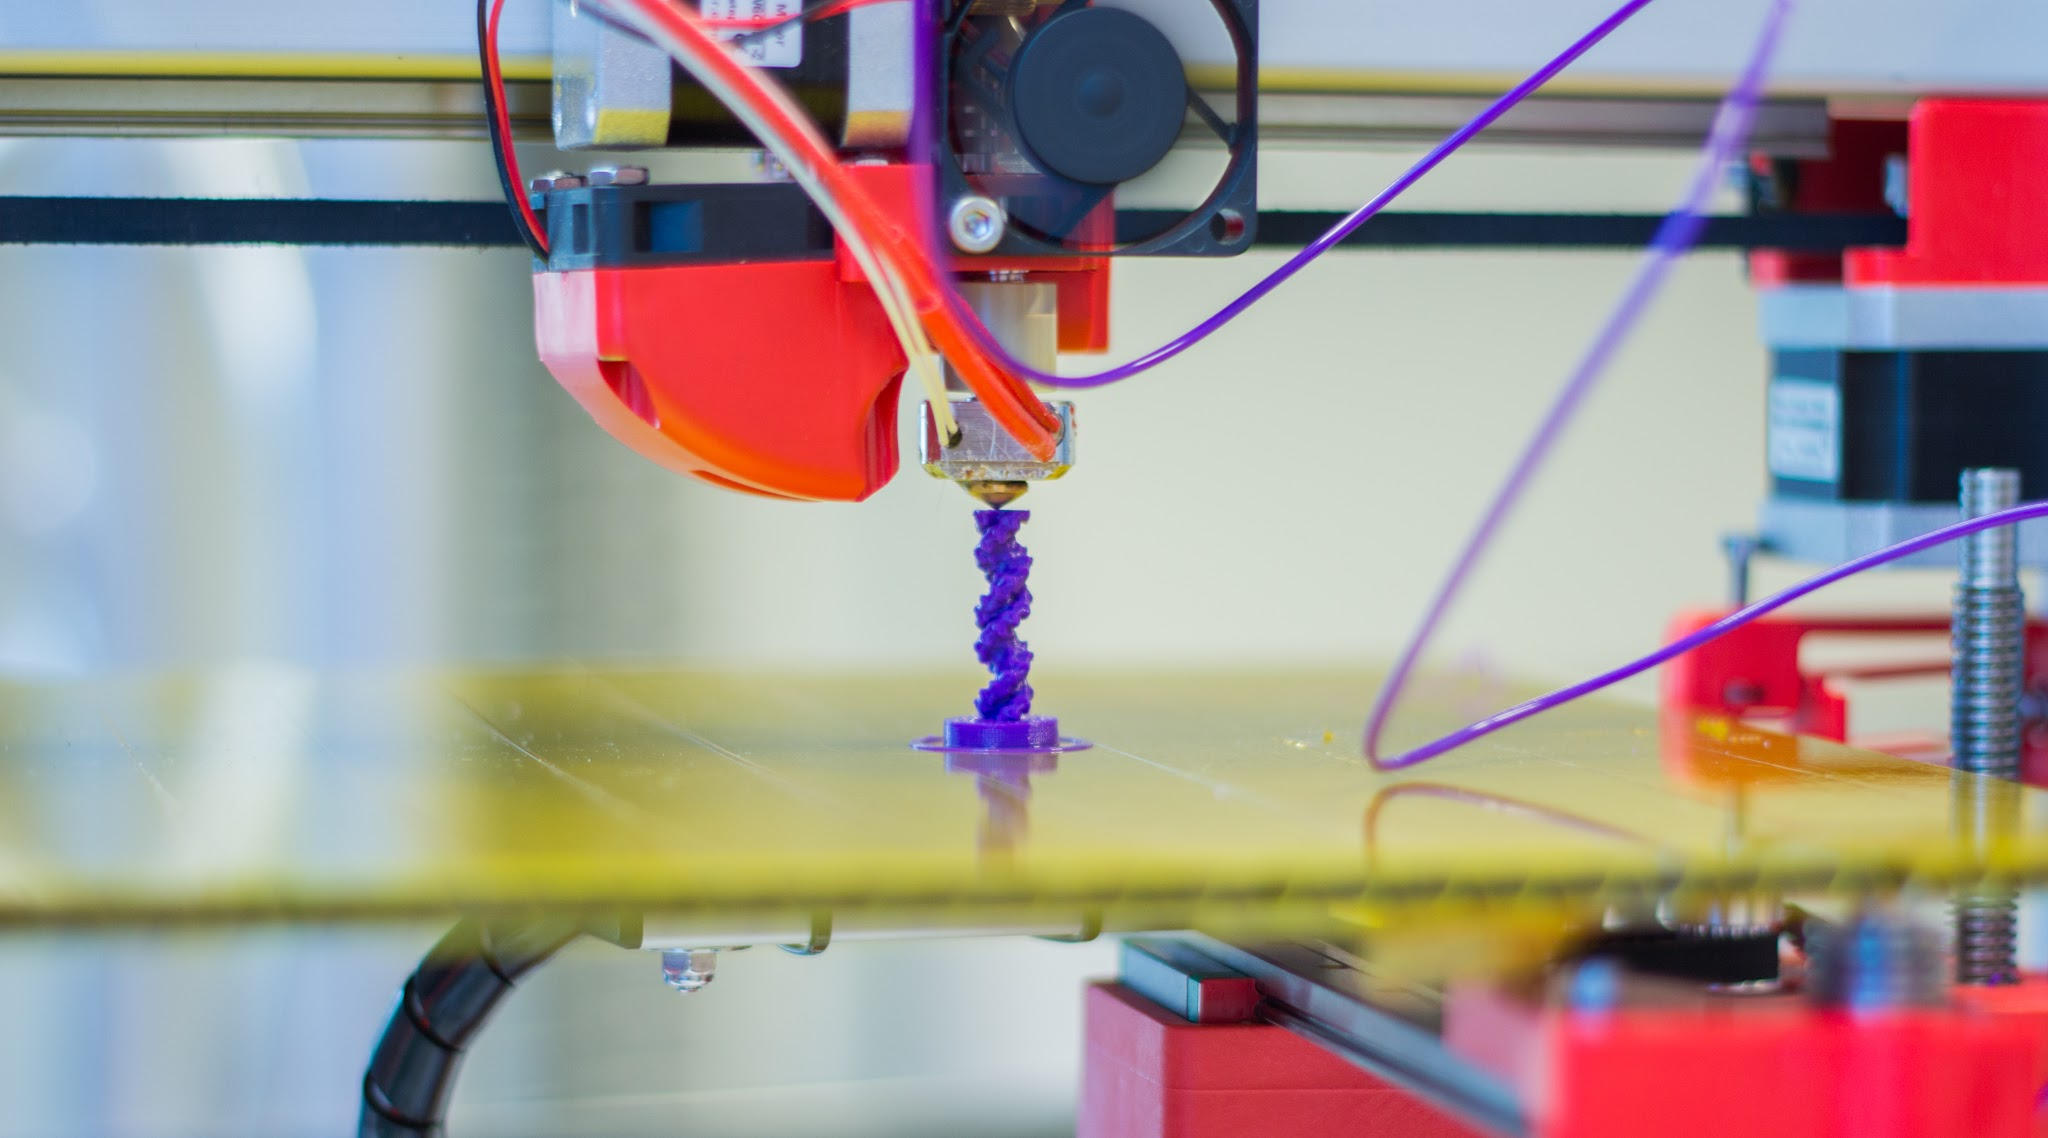
\includegraphics[width=.9\linewidth]{Felix_3D_Printer_-_Printing_Head.JPG}
\end{center}
\end{frame}
\begin{frame}[label={sec:org0e6d1fc}]{\ldots{}wait?}
\begin{block}{}
Something occurs to you
\end{block}
\end{frame}
\begin{frame}[label={sec:orge643353}]{Finite programs}
\begin{block}{}
Finite keyboards + finite length = countable number of programs
\end{block}
\end{frame}
\begin{frame}[label={sec:orgadc44d3}]{Reals and Integers}
\begin{block}{All the real numbers between 0 and 1}
\begin{center}
\begin{tabular}{lllll}
\(a_1\) & \(a_2\) & \(a_3\) & \(a_4\) & \ldots{}\\
\(b_1\) & \(b_2\) & \(b_3\) & \(b_4\) & \ldots{}\\
\(c_1\) & \(c_2\) & \(c_3\) & \(c_4\) & \ldots{}\\
\(d_1\) & \(d_2\) & \(d_3\) & \(d_4\) & \ldots{}\\
\ldots{} & \ldots{} & \ldots{} & \ldots{} & \ldots{}\\
\end{tabular}
\end{center}
\end{block}
\end{frame}
\begin{frame}[label={sec:orga059993}]{A table of programs}
\end{frame}
\begin{frame}[label={sec:org31e98b8}]{If we fuss with the diagonal}
\end{frame}
\begin{frame}[label={sec:orgd75fb14}]{A program that can't exist}
\end{frame}
\begin{frame}[label={sec:org2489ca5}]{You wake up}
\end{frame}
\begin{frame}[label={sec:org75bb20e}]{The Real World: Programming is \alert{hard}}
\end{frame}
\begin{frame}[label={sec:org88b31cc}]{The Real World: Programming is \alert{finite}}
\begin{block}{The finite nature of}
\end{block}
\end{frame}
\begin{frame}[label={sec:org1c34829}]{Thank you}
\begin{block}{}
{\Huge
Thank you for coming out!
}
\end{block}
\end{frame}
\end{document}